\documentclass[12pt]{article}
\usepackage[a4paper,  fancysections,  titlepage]{polytechnique}
\usepackage{amsmath,bm,empheq,graphicx,hyperref,upgreek,xcolor}
\usepackage[italicdiff]{physics}
\usepackage[justification=centering]{caption}

\hypersetup{colorlinks=true, urlcolor=cyan}
\newcommand{\ddfrac}[2]{{\displaystyle\frac{\displaystyle #1}{\displaystyle #2}}}

\title{Quantum Criticallity in Cuprates: PRL Report}
\author{Matéo Rivera, Saleh Shamloo Ahmadi\\Supervisor: Gaël Grissonnanche}
\date{March 15, 2025}

\begin{document}
\maketitle
\begin{abstract}

\end{abstract}
\section{Introduction}
\subsection{Cuprates: High-Temperature Superconductors}
Cuprates are a class of superconductors with high critical temperature that have been subject
to intense research since their discovery in 1986. They exhibit rich physical behavior, specially
in their various phases.

\begin{figure}
    \centering
    \includegraphics[width=0.5\textwidth]{figures/cuprate_structure}
    \caption{Crystal structure of a Cuprate (YBCO)}
    \label{fig:cuprate_structure}
\end{figure}

The origin of their superconductivity is still a mystery, but it is believed to be related to the
quantum critical point (QCP) that is present in the phase diagram of these materials. The existence
of this QCP is the subject of this research project.

\begin{figure}
    \centering
    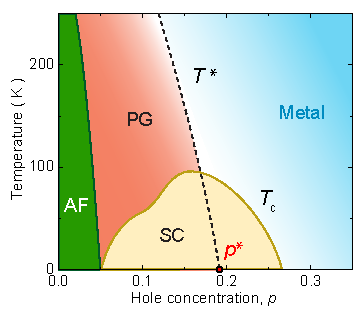
\includegraphics[width=0.5\textwidth]{figures/phase_diagram}
    \caption{Phase diagram of Cuprates}
    \label{fig:phase_diagram}
\end{figure}

A quantum critical point is a point in the phase diagram of a material where it goes through a phase
transition at zero temperature. In Cuprates, the phase transition occurs by increasing the doping
level of the material.

\subsection{Evidence for the QCP: Specific Heat}
In their 2019 paper, Michon et al. measured the specific heat of LSCO Cuprates and found a peak
in the specific heat at the critical doping level. This peak is a signature of the QCP.

\subsection{Evidence against the QCP: Optical Conductivity}
In their 2022 paper, Legros et al. measured the optical conductivity of LSCO Cuprates and, contrary
to the specific heat results, found no evidence of a QCP in the optical conductivity.

They used the Drude model to fit the optical conductivity and extracted the cyclotron mass.
They argue this is the same as the effective mass of the charge carriers, which is proportional to
the specific heat and is expected to diverge at the QCP. They found a simple linear dependence of
the cyclotron mass with the doping level, which contradicts the specific heat results.

We believe the use of the Drude model is not appropriate in this case, because it works well when
the Fermi surface is roughly isotropic, but we have a highly anisotropic Fermi surface in Cuprates.
We propose to use the Boltzmann transport equation to fit the optical conductivity and extract the
effective mass of the charge carriers.

\section{Methods}
\subsection{Reproduction of Drude Fits}

\subsection{Bolzmann Transport and Chambers Formula for Optical Conductivity}

\subsection{Fitting Procedure}

\section{Results}

\end{document}
